\documentclass[11pt, letterpaper]{article}
\usepackage[utf8]{inputenc}
\usepackage[letterpaper, margin=0.5in]{geometry}
\usepackage{amsmath}
\usepackage{amssymb}
\usepackage{amsthm}
\usepackage{graphicx}
\usepackage{listings}
\usepackage[font=scriptsize]{caption}
\usepackage{subcaption}
\usepackage{xcolor}

\newtheorem{lemma}{Lemma}
\newcommand{\indep}{\perp \!\!\! \perp}

\definecolor{codegreen}{rgb}{0,0.6,0}
\definecolor{codegray}{rgb}{0.5,0.5,0.5}
\definecolor{codepurple}{rgb}{0.58,0,0.82}
\definecolor{backcolour}{rgb}{0.95,0.95,0.92}

\lstdefinestyle{mystyle}{
    backgroundcolor=\color{backcolour},   
    commentstyle=\color{codegreen},
    keywordstyle=\color{magenta},
    numberstyle=\tiny\color{codegray},
    stringstyle=\color{codepurple},
    basicstyle=\ttfamily\footnotesize,
    breakatwhitespace=false,
    texcl=true,
    mathescape=true,
    breaklines=true,                 
    captionpos=b,                    
    keepspaces=true,                 
    numbers=left,                    
    numbersep=5pt,                  
    showspaces=false,                
    showstringspaces=false,
    showtabs=false,                  
    tabsize=2
}

\lstset{style=mystyle}
\graphicspath{ {../statics/} }
\captionsetup{justification=raggedright, singlelinecheck=false}

\author{Ryan Tang}
\title{STA 532 HW 3}
\date{February 5th 2023}

\begin{document}
\maketitle

\section{Ex 6}
\paragraph{(a)} Sum of two independent normal is normal
\begin{align*}
    X &\thicksim N(\mu_1, \Sigma_1), Y\thicksim N(\mu_2, \Sigma_2) \\
    E[e^{t^{\intercal}{X+Y}}] &= E[e^{t^{\intercal}X}]E[e^{t^{\intercal}Y}] \\
        &= \exp[t^{\intercal}\mu_1 + \frac{1}{2}t^{\intercal}\Sigma_1 t] \exp[t^{\intercal}\mu_2 + \frac{1}{2}t^{\intercal}\Sigma_2 t] \\
        &= \exp[t^{\intercal}(\mu_1+\mu_2) + \frac{1}{2}t^{\intercal}(\Sigma_1+\Sigma_2) t] \\
    X+Y &\thicksim N(\mu_1+\mu_2, \Sigma_1+\Sigma_2)
\end{align*}
\paragraph{(b)} Cholesky Decomposition of Multivariate Normal
\begin{align*}
    Y &\thicksim N_d(\mu, \Sigma), \Sigma = AA^{\intercal} \\
    Y &= \mu + AZ, Z = (Z_1, \dots, Z_d)^{\intercal}, Z_i \thicksim_{iid} N(0, 1) \\
    Z &= A^{-1} (Y - \mu) \\
    |\frac{\partial Z}{\partial Y}| &= |A^{-1}| = |\Sigma|^{-1/2} \\
    p(z) &= \frac{1}{(2\pi)^{d/2}}\exp[-\frac{1}{2}||z||^2] \\
    p(y) &= \frac{1}{(2\pi)^{d/2}} |\Sigma|^{-1/2} \exp[-\frac{1}{2}(y-\mu)^{\intercal}A^{-\intercal}A^{-1}(y-\mu)] \\
        &= \frac{1}{(2\pi)^{d/2} |\Sigma|^{1/2}} \exp[-\frac{1}{2}(y-\mu)^{\intercal}\Sigma^{-1}(y-\mu)] \\
        &\thicksim N(y|\mu, \Sigma)
\end{align*}
\paragraph{(c)} Simple Normal Block Matrix
\begin{align*}
    X &\thicksim N(\mu, \Sigma), \Sigma = \begin{bmatrix}\Sigma_{11} & 0 \\ 0 & \Sigma_{22}\end{bmatrix} \\
    X &= \begin{bmatrix}x_1 & x_2\end{bmatrix}, \mu = \begin{bmatrix}\mu_1 & \mu_2\end{bmatrix} \\
    \Lambda &= \Sigma^{-1} = \begin{bmatrix}\Sigma_{11}^{-1} & 0 \\ 0 & \Sigma_{22}^{-1}\end{bmatrix} \\
    p(x) &= (2\pi)^{-1/2} |\Sigma|^{-1/2} \exp\left[ -\frac{1}{2}(x-\mu)^{\intercal}\Lambda(x-\mu) \right] \\
        &\propto \exp\left[ -\frac{1}{2}[
            (x_1-\mu_1)^{\intercal}\Sigma_{11}^{-1}(x_1-\mu_1)
            + (x_2-\mu_2)^{\intercal}\Sigma_{22}^{-1}(x_2-\mu_2)
          ] \right] \\
        &= N(x_1|\mu_1, \Sigma_{11}) N(x_2|\mu_2, \Sigma_{22})
\end{align*}
\paragraph{(d)} Gaussian independence implies uncorrelated

We can see it through the use of moment generating function considering a bivariate normal joint with a simple covariance matrix. The only time the two marginals are independent is when $\phi = 0$, which means 0 covariances.
\begin{align*}
    X &= (x_1, x_2)^{\intercal} \thicksim N(\begin{bmatrix}\mu_1 \\ \mu_2\end{bmatrix}, \begin{bmatrix}1 & \phi \\ \phi & 1\end{bmatrix}) \\
    E[e^{t^{\intercal}X}] &= \exp\left[t^{\intercal}\mu + t^{\intercal}\Sigma t \right] \\
        &= \exp\left[ t_1\mu_1 + \frac{1}{2}t_1^2 + t_2\mu_2 + \frac{1}{2}t_2^2 + \phi t_1 t_2 \right] \\
        &= E[e^{t_1x_1}]E[e^{t_2x_2}]\exp[\phi t_1 t_2]
\end{align*}

\newpage
\section{Ex 7}
\paragraph{(a)} Proof X and Z are independent standard normal
\begin{align*}
    (x, y)^{\intercal} &\thicksim N(0, \Sigma=\begin{bmatrix}1 & \rho \\ \rho & 1\end{bmatrix}) \\
    z &= (y - \rho x) (1-\rho^2)^{-1/2} \\
    y &= (1-\rho^2)^{1/2} z + \rho x \\
    |\frac{\partial y}{\partial z}| &= (1-\rho^2)^{1/2} \\
    |\Sigma|^{-1/2} &= (1-\rho^2)^{-1/2}, \Lambda = \Sigma^{-1} = (1-\rho^2)^{-1} \begin{bmatrix}1 & -\rho \\ -\rho & 1\end{bmatrix} \\
    p(x,y) &= (2\pi)^{-1}(1-\rho^2)^{-1/2} \exp\left[ -\frac{1}{2(1-\rho^2)}(x^2+y^2-2\rho x y) \right] \\
    p(x,z) &= p(x, y=(1-\rho^2)^{1/2} z + \rho x) |\frac{\partial y}{\partial z}| \\
        &= (2\pi)^{-1} \exp\left[-\frac{1}{2}(x^2 + z^2) \right] \\
        &= N(x|0, 1) N(z|0, 1)
\end{align*}
\paragraph{(b)}
Based on the information given $W = (X, Y, X^2, Y^2, XY)^{\intercal}$, where $(x, y)^{\intercal} &\thicksim N(0, \Sigma=\begin{bmatrix}1 & \rho \\ \rho & 1\end{bmatrix})$. Hence, the marginal $X, Y$ are both standard normal $N(0, 1)$. 
\begin{align*}
    E[W] &= \begin{bmatrix}0 \\ 0 \\ 1 \\ 1 \\ \rho\end{bmatrix} \\
    Var[W] &=
      \begin{bmatrix}
        1 & \rho & 0 & 0 & 0 \\
        \rho & 1 & 0 & 0 & 0 \\
        0 & 0 & 2 & 2\rho+\rho^2-1 & 2\rho \\
        0 & 0 & 2\rho+\rho^2-1 & 2 & 2\rho \\
        0 & 0 & 2\rho & 2\rho & 2\rho \\
      \end{bmatrix} \\
    E[Y|X] &= \rho X, \quad E[X|Y] = \rho Y \\
    Var[Y|X] &= 1 - \rho^2 = Var[X|Y] \\
    E[XY] &= E[X E[Y|X]] = E[\rho X^2] = \rho \\
    Var[X^2] &= E[X^4] - E[X^2]^2 = 3-1 = 2 \\
    Var[XY] &= Var[X E[Y|X]] + E[X Var[Y|X]] = Var[\rho X^2] + E[X(1-\rho^2)] = 2\rho \\
    Cov(X^2, Y^2) &= E[(XY)^2] - E[X^2]E[Y^2] = Var[XY] + E[XY]^2 - E[X^2]E[Y^2] = 2\rho + \rho^2 - 1 \\
\end{align*}

\newpage
\section{EX 9}
We like to do a simulation-based experiment to test whether $R_n/\log_2{n} \xrightarrow{p} 1$. Where $R_n$ is the longest consecutive heads in n coin flips. Following the definition of convergence in probability, the above expression is equivalent to the following in the limit, with $\epsilon$ being any positive real number.
\begin{align*}
    \lim_{n \rightarrow \infty} &\text{Pr} \left( |\frac{R_n}{\log_2{n}} - 1| > \epsilon \right) = 0 \\
    Z &= I(|\frac{R_n}{\log_2{n}} - 1| > \epsilon) \\
    \lim_{n \rightarrow \infty} &\mathbf{E}[Z|n, \epsilon] = 0 \\
    Z_i|n, \epsilon &\thicksim_{iid} Bernoulli(p)
\end{align*}

The tricky part of experimenting is that $R_n$ is a random variable, so there is an unavoidable measurement error in the samples while evaluating the expectation. However, given $n, \epsilon$, we can draw IID samples $Z_i|n, \epsilon$, so the expectation converges to a normal distribution in the limit. Then, what is left is a trivial t-test on some confidence interval. The actual experiment result is shown in the below chart. We can observe the limiting behavior in which the expectation converges to 0 asymptotically.

\begin{figure*}[!h]
  \centering
  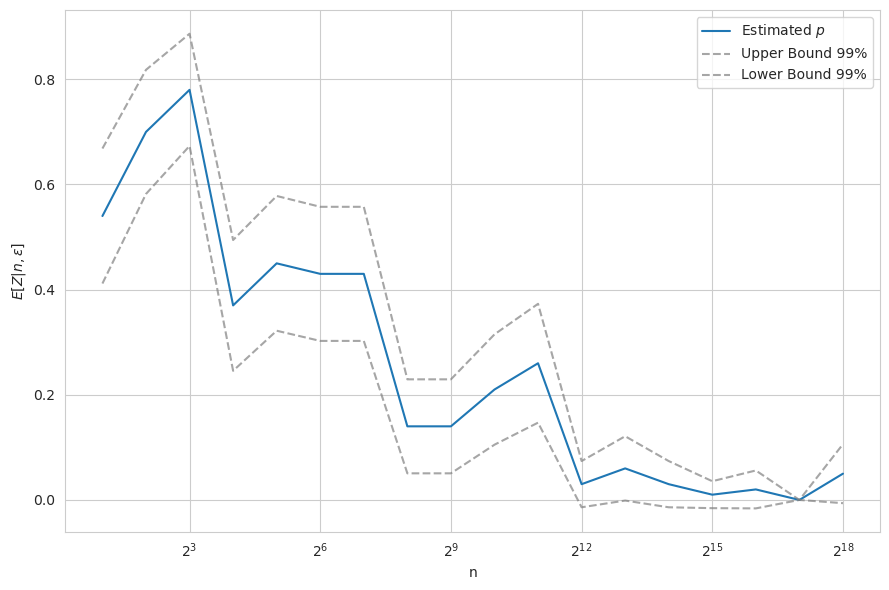
\includegraphics[width=0.75\textwidth]{hw3-1.png}
  \captionsetup{justification=centering}
  \caption{$\epsilon = 0.25$, for every $n$, the experiment is repeated 100 times, which was how the confidence intervals were constructed.}
\end{figure*}

\end{document}